% =====================================================================
\chapter{HIỆN THỰC HỆ THỐNG THEO USE CASE}\label{chap:hienthuc}
% =====================================================================

Chương này trình bày quá trình hiện thực theo đúng thứ tự 10 use case ở
Bảng~\ref{tab:uc-summary}. Mỗi mục mở đầu bằng bảng đặc tả use case gồm tác nhân, mục tiêu,
tiền điều kiện, sự kiện kích hoạt, luồng chính, luồng ngoại lệ và hậu điều kiện; phần tiếp
theo phân tích cách hiện thực trên vi điều khiển và lý do chọn các thông số. Kết quả kiểm thử
tương ứng được tổng hợp ở Chương~\ref{chap:kiemthu}.

\section{UC01. Xem chỗ trống tại cổng}\label{sec:uc01}
Use case này giúp người lái quyết định có vào bãi hay không và cần đi tới ô nào. Đặc tả của use
case được trình bày ở Bảng~\ref{tab:uc01}.

\begin{ucspec}{Đặc tả UC01. Xem chỗ trống tại cổng}{tab:uc01}
Tác nhân chính & Người lái xe \\ \midrule
Tác nhân phụ & Sensor Client \\ \midrule
Mục tiêu & Biết số chỗ trống và vị trí từng chỗ trống trước khi vào bãi \\ \midrule
Tiền điều kiện & Máy chủ và Sensor Client đã kết nối vào mạng Wi-Fi \\ \midrule
Kích hoạt & Một xe đi vào hoặc rời khỏi một ô đỗ \\ \midrule
Luồng chính &
\bul Cảm biến hồng ngoại của ô đổi mức logic.
\bul Sensor Client lọc nhiễu 50\,ms rồi gửi ngay bản tin \code{parking\_update}.
\bul Máy chủ kiểm tra bản tin, cập nhật trạng thái bãi và đánh thức tác vụ màn hình.
\bul Màn hình tại cổng hiển thị số chỗ trống và năm ô S1 đến S5, vạch xanh cho ô trống, vạch đỏ cho ô có xe.
\bul Người lái đọc thông tin trên màn hình. \\ \midrule
Luồng ngoại lệ &
\bul Gói tin bị mất: bản tin nhắc lại sau tối đa 1\,s cập nhật lại trạng thái.
\bul Bản tin sai định dạng: máy chủ bỏ qua và giữ trạng thái cũ.
\bul Sensor Client im lặng quá 3\,s: màn hình hiển thị \code{SENSOR OFFLINE}, năm ô chuyển xám. \\ \midrule
Hậu điều kiện & Màn hình phản ánh đúng trạng thái năm ô đỗ với độ trễ khoảng 0,1\,s \\
\end{ucspec}

Bước lọc nhiễu trong luồng chính là cần thiết vì mép xe và bánh xe làm tín hiệu hồng ngoại bật
tắt liên tục trong vài chục mili giây khi xe đang lăn vào ô. Hình~\ref{fig:debounce} minh họa
thuật toán: mỗi cảm biến có bộ đếm thời gian riêng, mức mới chỉ được chấp nhận khi giữ nguyên đủ
50\,ms.

\begin{figure}[H]
\centering
\begin{tikzpicture}[x=0.9cm,y=0.6cm,font=\scriptsize]
\node[anchor=east] at (-0.2,2.5) {Tín hiệu thô};
\draw[thick] (0,2) -- (2,2) -- (2,3) -- (2.3,3) -- (2.3,2) -- (2.5,2) -- (2.5,3) -- (2.7,3) -- (2.7,2) -- (2.9,2) -- (2.9,3) -- (11,3);
\node[anchor=east] at (-0.2,0.5) {Trạng thái};
\draw[thick,accent] (0,0) -- (3.9,0) -- (3.9,1) -- (11,1);
\draw[dashed,gray] (2.9,3.3) -- (2.9,-0.4);
\draw[dashed,gray] (3.9,3.3) -- (3.9,-0.4);
\draw[{Stealth}-{Stealth}] (2.9,-0.6) -- node[below]{ổn định 50\,ms} (3.9,-0.6);
\node[align=center] at (2.45,3.8) {nhiễu khi xe\\đang lăn vào};
\node[draw,fill=boxB,align=center] at (7.5,-0.9) {gửi \code{parking\_update} ngay};
\draw[-{Stealth},thick] (3.9,1) to[bend right=10] (6.2,-0.6);
\end{tikzpicture}
\caption{Lọc nhiễu tín hiệu cảm biến ô đỗ}\label{fig:debounce}
\end{figure}

Thời gian 50\,ms được tinh chỉnh thực nghiệm từ giá trị ban đầu 250\,ms: đủ loại bỏ nhiễu mà
vẫn tạo cảm giác tức thời. Ngoài việc gửi ngay khi có thay đổi, Sensor Client còn nhắc lại
toàn bộ trạng thái mỗi giây; nhờ vậy, một gói UDP bị mất chỉ gây sai lệch tối đa một giây và
tự được sửa ở lần gửi sau, không cần cơ chế truyền lại.

Ở phía máy chủ, tác vụ \code{udp\_server} đánh thức tác vụ màn hình bằng thông báo tác vụ
ngay khi có dữ liệu mới. Màn hình dùng một bộ đệm khung $240\times240$ điểm ảnh 16 bit
(115\,200 byte): toàn bộ giao diện được vẽ vào RAM rồi truyền một lần qua SPI 40\,MHz có DMA,
mất khoảng 23\,ms. Tần số 40\,MHz bằng đúng một nửa xung nhịp 80\,MHz của khối SPI và thấp hơn
giới hạn khoảng 62\,MHz của ST7789, chừa biên an toàn cho dây nối. Giao diện thực tế ở
Hình~\ref{fig:tft-live} gồm hàng trên là số chỗ trống, ô nhiệt độ và ô mực nước kèm một ảnh
động trang trí; hàng giữa là năm ô đỗ; vùng chân màn hình dành cho hóa đơn và thông báo. Khi
Sensor Client mất kết nối, dữ liệu cũ không còn được dùng để từ chối thẻ hay phát cảnh báo,
tránh việc hệ thống hành động dựa trên trạng thái không còn đúng.

\section{UC02. Gửi xe bằng thẻ RFID}\label{sec:uc02}
Use case này mô tả một lượt xe vào bãi, bao gồm cả các trường hợp hệ thống phải từ chối. Đặc tả
được trình bày ở Bảng~\ref{tab:uc02}.

\begin{ucspec}{Đặc tả UC02. Gửi xe bằng thẻ RFID}{tab:uc02}
Tác nhân chính & Người lái xe \\ \midrule
Tác nhân phụ & RFID Client, Đồng hồ hệ thống \\ \midrule
Mục tiêu & Được mở cổng vào và bắt đầu tính thời gian gửi xe \\ \midrule
Tiền điều kiện & Thẻ chưa có phiên gửi xe; bãi còn chỗ; không có cảnh báo ngập \\ \midrule
Kích hoạt & Người lái đưa thẻ vào đầu đọc ở cổng vào \\ \midrule
Luồng chính &
\bul RFID Client đọc mã UID và gửi \code{rfid\_event} với \code{"gate":"in"} kèm số thứ tự \code{seq}.
\bul Máy chủ trả gói xác nhận, tạo phiên mới, lưu thời điểm vào, ghi nhật ký \code{IN} và lưu bảng phiên vào flash.
\bul Máy chủ mở thanh chắn cổng vào và hẹn giờ 3\,s.
\bul Xe đi qua cổng; hết 3\,s, thanh chắn hạ xuống khi cảm biến hồng ngoại ở cổng xác nhận làn trống. \\ \midrule
Luồng ngoại lệ &
\bul Thẻ đã có phiên trong bãi: không mở cổng, màn hình báo \code{WRONG GATE} và gợi ý dùng cổng ra trong 5\,s.
\bul Bãi đã đủ 5 phiên hoặc cảm biến báo đủ 5 ô có xe: không mở cổng, màn hình báo \code{PARKING FULL}.
\bul Đang có cảnh báo ngập: không mở cổng, màn hình báo \code{FLOOD ALARM - ENTRY CLOSED}.
\bul Gói tin bị mất: sau 300\,ms chưa có xác nhận, RFID Client gửi lại, tối đa 6 lần; máy chủ nhận ra bản gửi lại qua \code{seq} nên không mở cổng lần hai.
\bul Xe còn nằm dưới cần chắn khi hết 3\,s: thanh chắn giữ mở cho tới khi làn trống liên tục 1\,s.
\bul Một xe khác đi theo mà không quẹt thẻ: sau 15\,s số ô có xe vẫn nhiều hơn số thẻ, còi kêu ngắt quãng và màn hình báo \code{CAR W/O CARD}. \\ \midrule
Hậu điều kiện & Thẻ có phiên gửi xe, nhật ký có bản ghi \code{IN}, thanh chắn đóng \\
\end{ucspec}

Hình~\ref{fig:seq-rfid} biểu diễn trình tự trao đổi giữa các thành phần trong luồng chính, trường
hợp gói tin bị mất và luồng ra khi không bật thanh toán QR.

\begin{figure}[H]
\centering
\mmd[1][0.8]{seq_rfid}
\caption{Biểu đồ tuần tự gửi xe, xử lý mất gói và lấy xe}\label{fig:seq-rfid}
\end{figure}

\subsection{Đọc thẻ trên hai đầu đọc dùng chung bus}
RFID Client quét luân phiên hai đầu đọc và tại mỗi thời điểm chỉ bật ăng-ten của một đầu đọc.
Hai đầu đọc cùng tần số 13,56\,MHz đặt gần nhau sẽ gây nhiễu chéo nếu cùng phát, nên cách bật
luân phiên loại bỏ hoàn toàn vấn đề này. Sau khi bật ăng-ten, client chờ 4\,ms để thẻ thụ động
nhận đủ năng lượng; độ khuếch đại được đặt ở mức 48\,dB để bù tầm đọc khi đầu đọc nằm sau thành
hộp. Một thẻ để yên trên đầu đọc sẽ bị đọc liên tục, vì vậy client bỏ qua các lần đọc lặp lại
cùng một thẻ trong vòng 2\,s, tránh trường hợp một lần quẹt bị hiểu thành vào rồi ra. Mã UID được
đổi sang chuỗi hex trong bộ đệm cố định thay vì kiểu \code{String} của Arduino, để bộ nhớ heap
khoảng 80\,KB của ESP8266 không bị phân mảnh khi chạy lâu.

\subsection{Bảo đảm không mất lượt quẹt thẻ}
Khác với trạng thái cảm biến, sự kiện quẹt thẻ chỉ xảy ra một lần; mất gói đồng nghĩa với mất
lượt quẹt. Thay vì chuyển sang TCP, hệ thống bổ sung đúng phần độ tin cậy cần thiết như ở phần
giữa của Hình~\ref{fig:seq-rfid}. Máy chủ ghi nhớ 16 giá trị \code{seq} gần nhất; gặp lại một
\code{seq} đã xử lý, máy chủ hiểu đó là bản gửi lại, chỉ trả xác nhận mà không xử lý lần hai.
Giá trị \code{seq} khởi đầu từ một số ngẫu nhiên do bộ sinh số ngẫu nhiên phần cứng của ESP8266
tạo ra mỗi lần khởi động rồi tăng dần, nên client không cần lưu gì vào flash.

\subsection{Điều khiển thanh chắn}
Servo SG90 nhận xung chu kỳ 20\,ms, độ rộng xung quyết định góc quay như Hình~\ref{fig:pwm}.

\begin{figure}[H]
\centering
\begin{tikzpicture}[x=0.55cm,y=0.7cm,font=\scriptsize]
\draw[-{Stealth}] (0,0) -- (23,0) node[right]{$t$ (ms)};
\draw[-{Stealth}] (0,0) -- (0,1.8) node[left]{PWM};
\draw[thick,accent] (0,0) -- (0,1.2) -- (1.45,1.2) -- (1.45,0) -- (20,0) -- (20,1.2) -- (21.45,1.2) -- (21.45,0) -- (22.5,0);
\draw[{Stealth}-{Stealth}] (0,-0.5) -- node[below]{chu kỳ $T = 20$\,ms (50\,Hz)} (20,-0.5);
\draw[{Stealth}-{Stealth}] (0,1.5) -- node[above]{$p$} (1.45,1.5);
\node[align=left,anchor=west] at (3,1.0) {$p = 500$\,µs $\to 0°$\quad $p = 1450$\,µs $\to 90°$\quad $p = 2400$\,µs $\to 180°$};
\end{tikzpicture}
\caption{Dạng xung điều khiển servo SG90}\label{fig:pwm}
\end{figure}

Từ Hình~\ref{fig:pwm}, độ rộng xung $p$ ứng với góc $\theta$ và giá trị $D$ nạp vào thanh ghi
của khối LEDC 14 bit được tính theo
\begin{equation}
  p(\theta) = 500 + \frac{1900\,\theta}{180}\ \text{µs}, \qquad
  D = \left\lfloor \frac{p \cdot (2^{14}-1)}{20\,000} \right\rfloor .
\end{equation}
Với $\theta=90°$ ta có $p=1450$\,µs và $D=1187$; với $\theta=0°$ ta có $p=500$\,µs và $D=409$.
Độ phân giải 14 bit cho mỗi bước khoảng 1,22\,µs, tương đương 0,12°, mịn hơn nhiều so với vùng
chết khoảng 1° của SG90 nên servo không rung. Dải 500--2400\,µs là giá trị đo thực tế; dải danh
nghĩa 1000--2000\,µs không đủ để servo quay hết hành trình. Thanh chắn cổng ra được lắp đối xứng
nên góc mở và đóng đảo ngược so với cổng vào, khác biệt này chỉ được khai báo ở một hàm.

Việc đóng thanh chắn được hẹn bằng bộ hẹn giờ một lần \code{esp\_timer} thay vì một tác vụ hỏi
vòng: hàm đóng được gọi đúng thời điểm với sai số micro giây và CPU không bị đánh thức vô ích.
Hình~\ref{fig:fsm-gate} là máy trạng thái của một thanh chắn, dùng chung cho UC02, UC03, UC05 và
UC06.

\begin{figure}[H]
\centering
\begin{tikzpicture}[
  st/.style={draw=accent,fill=boxA,rounded corners=2pt,font=\footnotesize,align=center,minimum height=1cm,text width=2.6cm,inner sep=2pt},
  lb/.style={font=\scriptsize,align=center,inner sep=1.5pt},
  arr/.style={-{Stealth[length=2mm]},draw=black!70}]
\node[st] (D) at (0,0) {Đóng};
\node[st] (H) at (5,0) {Mở có hẹn giờ 3\,s};
\node[st,fill=boxC] (G) at (10.2,0) {Giữ mở\\xe còn trong cổng};
\node[st] (M) at (0,-3.4) {Mở thủ công};
\node[st,fill=boxD] (F) at (5,2.9) {Mở do cháy\\khóa lệnh đóng};
\fill (-2.2,0) circle (2pt); \draw[arr] (-2.2,0) -- (D);
\draw[arr] ([yshift=2mm]D.east) -- node[lb,above] {thẻ hợp lệ} ([yshift=2mm]H.west);
\draw[arr] ([yshift=-2mm]H.west) -- node[lb,below] {hết 3\,s, làn trống} ([yshift=-2mm]D.east);
\draw[arr] ([yshift=2mm]H.east) -- node[lb,above] {hết 3\,s, IR bị che} ([yshift=2mm]G.west);
\draw[arr] (G.south) -- ++(0,-1.3) -| node[lb,below,pos=0.25] {làn trống liên tục 1\,s} ([xshift=9mm]D.south);
\draw[arr] (G) edge[loop right,looseness=4] node[lb,right,text width=1.5cm] {kiểm tra mỗi 50\,ms} (G);
\draw[arr] ([xshift=-6mm]D.north) |- node[lb,above,pos=0.75] {có lửa (từ mọi trạng thái)} (F.west);
\draw[arr] (F.east) -| node[lb,above,pos=0.25] {hết lửa, kiểm tra IR} (G.north);
\draw[arr] ([xshift=-7mm]D.south) -- node[lb,left] {lệnh mở từ web} ([xshift=-7mm]M.north);
\draw[arr] ([xshift=1mm]M.north) -- node[lb,right,pos=0.3] {lệnh đóng từ web, làn trống} ([xshift=1mm]D.south);
\draw[arr] (M) edge[loop right,looseness=4] node[lb,right,text width=3.2cm] {lệnh đóng khi xe trong cổng: từ chối, mã 409} (M);
\end{tikzpicture}
\caption{Máy trạng thái của một thanh chắn}\label{fig:fsm-gate}
\end{figure}

Theo Hình~\ref{fig:fsm-gate}, khi hết 3\,s, hàm đóng đọc cảm biến hồng ngoại của cổng. Nếu tia
bị che, tức là xe còn nằm dưới cần chắn, thanh chắn được giữ mở và hàm đóng tự hẹn lại sau
50\,ms để kiểm tra tiếp. Thanh chắn chỉ hạ xuống khi tia thông suốt liên tục 1\,s; điều kiện liên
tục này loại bỏ trường hợp cảm biến nháy một mẫu đúng lúc khoảng trống giữa hai trục xe đi qua.
Logic đếm thời gian thông suốt được tách thành một hàm thuần không phụ thuộc phần cứng để kiểm
thử trên máy tính. Vì một lệnh khác có thể xảy ra đồng thời với hàm đóng, hàm đóng kiểm tra lại
hạn đóng trong vùng bảo vệ bởi mutex. Cả hai thanh chắn luôn khởi động ở vị trí đóng, vì vậy
trạng thái thanh chắn không cần lưu vào flash.

\subsection{Từ chối lượt quẹt không hợp lệ}
Các luồng ngoại lệ từ chối của UC02 và UC03 cùng dựa trên trạng thái của thẻ.
Hình~\ref{fig:fsm-card} tổng hợp các trạng thái của một thẻ và các chuyển trạng thái, bao gồm cả
các nhánh bị từ chối.

\begin{figure}[H]
\centering
\begin{tikzpicture}[
  st/.style={draw=accent,fill=boxA,rounded corners=2pt,font=\footnotesize,align=center,minimum height=0.95cm,text width=2.05cm,inner sep=2pt},
  wide/.style={st,text width=2.9cm},
  lb/.style={font=\scriptsize,align=center,text width=3.3cm,inner sep=2pt},
  arr/.style={-{Stealth[length=2mm]},draw=black!70}]
\node[st] (N) at (-5.6,0) {Thẻ ngoài bãi};
\node[st] (T) at (-0.6,0) {Thẻ trong bãi};
\node[wide] (C) at (5.4,0) {Chờ thanh toán\\QR trên TFT, cổng đóng};
\node[wide,text width=3.3cm] (R1) at (-5.6,4.3) {Bị từ chối\\WRONG GATE / FULL};
\node[wide] (R2) at (-0.6,4.3) {Bị từ chối\\WRONG GATE};
\fill (-7.5,0) circle (2pt);
\draw[arr] (-7.5,0) -- (N.west);
\draw[arr] ([yshift=2.5mm]N.east) -- node[lb,above,text width=2.7cm] {quẹt cổng vào, còn chỗ\\mở cổng vào} ([yshift=2.5mm]T.west);
\draw[arr] ([yshift=-2.5mm]T.west) -- node[lb,below,text width=2.7cm] {quẹt cổng ra, tắt QR\\tính phí, mở cổng ra} ([yshift=-2.5mm]N.east);
\draw[arr] (T.east) -- node[lb,above,text width=3.2cm] {quẹt cổng ra, bật QR\\chốt phí} (C.west);
\draw[arr] ([xshift=-7mm]C.north) .. controls +(-0.2,1.1) and +(0.2,1.1) .. node[lb,above,pos=0.5,text width=2.9cm] {quẹt lại, hiện lại QR cũ} ([xshift=7mm]C.north);
\draw[arr] ([xshift=-3.5mm]T.north) -- node[lb,left,pos=0.68,text width=1.9cm] {quẹt cổng vào} ([xshift=-3.5mm]R2.south);
\draw[arr] ([xshift=3.5mm]R2.south) -- node[lb,right,pos=0.32,text width=1.9cm] {thông báo 5\,s} ([xshift=3.5mm]T.north);
\draw[arr] ([xshift=-3.5mm]N.north) -- node[lb,left,pos=0.68,text width=1.6cm] {quẹt cổng ra, hoặc bãi đầy} ([xshift=-3.5mm]R1.south);
\draw[arr] ([xshift=3.5mm]R1.south) -- node[lb,right,pos=0.32,text width=1.9cm] {thông báo 5\,s} ([xshift=3.5mm]N.north);
\draw[arr] (C.south) -- ++(0,-1.7) -| node[lb,below,pos=0.25,text width=8cm] {SePay khớp giao dịch hoặc người vận hành xác nhận, mở cổng ra} (N.south);
\end{tikzpicture}
\caption{Máy trạng thái của một thẻ RFID}\label{fig:fsm-card}
\end{figure}

Hình~\ref{fig:fsm-card} cho thấy hai trạng thái bị từ chối đều tự quay về trạng thái trước đó sau
5\,s, nghĩa là lần quẹt sai không làm thay đổi phiên gửi xe; nếu ngay sau đó có một lần quẹt hợp
lệ, thông báo cũ bị xóa ngay để không che thông tin mới. Điều kiện bãi đầy được xét theo cả số
phiên lẫn số ô có xe theo cảm biến, nên hệ thống vẫn từ chối thẻ mới khi có xe đã vào mà không
quẹt thẻ. Trường hợp xe đi theo không quẹt thẻ được phát hiện bằng cách so sánh liên tục hai số
này; ngưỡng 15\,s đủ dài để một xe vừa quẹt thẻ có thời gian đi vào ô mà không gây báo động nhầm.

\section{UC03. Thanh toán phí và lấy xe}\label{sec:uc03}
Use case này mô tả một lượt xe ra bãi khi bật thanh toán VietQR. Đặc tả được trình bày ở
Bảng~\ref{tab:uc03}.

\begin{ucspec}{Đặc tả UC03. Thanh toán phí và lấy xe}{tab:uc03}
Tác nhân chính & Người lái xe \\ \midrule
Tác nhân phụ & RFID Client, SePay, Đồng hồ hệ thống \\ \midrule
Mục tiêu & Trả đúng phí gửi xe bằng chuyển khoản và được mở cổng ra \\ \midrule
Tiền điều kiện & Thẻ đang có phiên gửi xe; tài khoản nhận và khóa truy cập SePay đã được cấu hình \\ \midrule
Kích hoạt & Người lái đưa thẻ vào đầu đọc ở cổng ra \\ \midrule
Luồng chính &
\bul Máy chủ tính thời gian gửi và phí, chốt phí, tạo mã thanh toán gồm tiền tố \code{PK} và 6 ký tự.
\bul Thanh chắn vẫn đóng; màn hình hiển thị mã VietQR, số tiền và nội dung chuyển khoản.
\bul Người lái quét mã bằng ứng dụng ngân hàng và chuyển khoản với số tiền đã điền sẵn.
\bul Máy chủ truy vấn SePay mỗi 3\,s và tìm thấy giao dịch khớp mã và đúng số tiền.
\bul Máy chủ đóng phiên, ghi nhật ký \code{OUT}, cộng doanh thu; màn hình hiển thị lời cảm ơn 5\,s rồi hóa đơn 60\,s.
\bul Thanh chắn cổng ra mở và đóng theo cùng điều kiện cảm biến cổng như UC02. \\ \midrule
Luồng ngoại lệ &
\bul Thẻ chưa có phiên gửi xe: không mở cổng, màn hình báo \code{WRONG GATE} và gợi ý dùng cổng vào.
\bul Người lái quẹt lại cùng thẻ: màn hình hiển thị lại đúng mã QR cũ, thời gian chờ được tính lại.
\bul Xe khác quẹt khi lượt trước còn hiệu lực: mã QR của xe trước được giữ, dòng cuối màn hình báo \code{NEXT CAR: WAIT, ONE IS PAYING}.
\bul Chuyển dư hoặc thiếu tiền: giao dịch không được chấp nhận, cổng vẫn đóng.
\bul Quá 180\,s chưa nhận được tiền: màn hình báo \code{PAY AT BOOTH} trong 30\,s; tiếp tục ở UC04. \\ \midrule
Hậu điều kiện & Phiên được giải phóng; nhật ký có bản ghi \code{OUT}; doanh thu tăng đúng bằng phí \\
\end{ucspec}

Phí gửi xe được tính theo giờ, làm tròn lên và tối thiểu một giờ:
\begin{equation}
  \text{phí} = 5000 \times \max\left(1, \left\lceil \frac{t}{3600} \right\rceil\right)\ \text{VNĐ},
\end{equation}
trong đó $t$ là thời gian gửi tính bằng giây. Công thức được hiện thực bằng phép chia nguyên
\code{(t + 3599) / 3600} để tránh số thực, và bão hòa ở giá trị lớn nhất của kiểu 32 bit nếu tràn.
Mã thanh toán dùng 31 ký tự gồm chữ in hoa và chữ số, đã loại bỏ \code{I}, \code{L}, \code{O},
\code{0}, \code{1} vì dễ nhầm khi người lái phải gõ tay. Hình~\ref{fig:seq-pay} là trình tự trao
đổi trong quá trình thanh toán.

\begin{figure}[H]
\centering
\mmd[0.78][0.55]{seq_pay}
\caption{Biểu đồ tuần tự thanh toán VietQR ở cổng ra}\label{fig:seq-pay}
\end{figure}

\subsection{Sinh mã VietQR trên vi điều khiển}
Chuỗi VietQR được máy chủ tự dựng theo chuẩn của NAPAS, vốn là định dạng EMVCo: mỗi trường gồm
mã 2 chữ số, độ dài 2 chữ số và giá trị, các trường 38 và 62 chứa trường con theo cùng quy tắc.
Bảng~\ref{tab:vietqr} liệt kê các trường trong chuỗi do máy chủ sinh ra.

\begin{table}[H]
\centering\small
\caption{Cấu trúc chuỗi VietQR do máy chủ sinh}\label{tab:vietqr}
\begin{tabularx}{\linewidth}{@{}llX@{}}
\toprule
Mã & Trường & Giá trị \\ \midrule
00 & Phiên bản định dạng & \code{01} \\
01 & Kiểu mã & \code{12}, mã động dùng cho một số tiền cụ thể \\
38 & Thông tin người nhận & Định danh NAPAS \code{A000000727}, mã BIN ngân hàng và số tài khoản, dịch vụ \code{QRIBFTTA} \\
53, 58 & Tiền tệ, quốc gia & \code{704} (VNĐ), \code{VN} \\
54 & Số tiền & Phí đã chốt, ví dụ \code{10000} \\
62 & Dữ liệu bổ sung & Nội dung chuyển khoản là mã thanh toán, ví dụ \code{PK7XK2QM} \\
63 & Mã kiểm tra & CRC16-CCITT (đa thức \code{0x1021}, giá trị đầu \code{0xFFFF}) \\
\bottomrule
\end{tabularx}
\end{table}

Trường 54 trong Bảng~\ref{tab:vietqr} cố định số tiền đúng bằng phí, và trường 62 cố định nội
dung chuyển khoản là mã thanh toán. Hàm sinh chuỗi được kiểm chứng trùng từng byte với một mã
VietQR mẫu đã công bố và với giá trị kiểm tra chuẩn \code{0x29B1} của CRC16-CCITT. Mã QR được
vẽ bằng thư viện qrcodegen với mức sửa lỗi M; việc sinh mã hoàn toàn trên chip nên vẫn hoạt động
khi mất Internet. Nếu số tài khoản không hợp lệ hoặc để trống, máy chủ không vẽ mã QR mà hiển
thị \code{PAY AT BOOTH} và việc thu tiền chuyển sang UC04.

\subsection{Đối soát giao dịch qua SePay}
SePay theo dõi biến động số dư của tài khoản nhận và cho phép truy vấn giao dịch qua API. Khi
một lượt thanh toán bắt đầu, tác vụ \code{sepay} ghi lại mã giao dịch mới nhất, sau đó cứ 3\,s
truy vấn các giao dịch có mã lớn hơn, nên chỉ những giao dịch xảy ra sau khi hiển thị mã QR mới
được xét. Một giao dịch được chấp nhận khi nội dung chứa mã thanh toán và số tiền đúng bằng phí;
chuyển dư hay thiếu đều không mở cổng, vì mã QR chỉ điền sẵn số tiền còn việc khóa ô nhập là do
từng ứng dụng ngân hàng quyết định. Thử nghiệm thực tế cho thấy một số ví điện tử như MoMo thay
nội dung chuyển khoản bằng nội dung riêng, do đó máy chủ chấp nhận thêm giao dịch vào đúng tài
khoản nhận với số tiền đúng bằng phí. Vì mỗi lúc chỉ có một xe thanh toán và chỉ xét giao dịch
sau thời điểm hiện mã, cách đối soát này không nhầm lẫn giữa các xe.

Máy chủ dùng phương pháp hỏi vòng thay vì webhook vì ESP32-C3 nằm sau NAT của router, không có
địa chỉ để Internet gọi tới. Chu kỳ 3\,s cho độ trễ vài giây, thấp hơn nhiều so với giới hạn
2--3 yêu cầu mỗi giây của SePay. Kết nối HTTPS cần thêm bộ nhớ cho TLS trong khi RAM đã chật bởi
bộ đệm khung 115\,KB; vì vậy bộ đệm TLS chỉ được cấp phát trong lúc gửi yêu cầu, và tác vụ ảnh
động trả lại hai bộ đệm 18\,KB của nó trong lúc có xe đang thanh toán, khi ảnh động vốn không
hiển thị.

\section{UC04. Xác nhận thanh toán tại quầy}\label{sec:uc04}
Thanh toán tự động phụ thuộc vào Internet, dịch vụ SePay và việc người lái chuyển khoản đúng.
Khi một trong các điều kiện này không thỏa mãn, hoặc khi người lái trả tiền mặt, bãi vẫn phải
cho xe ra. Bảng~\ref{tab:uc04} đặc tả use case dành cho tình huống này.

\begin{ucspec}{Đặc tả UC04. Xác nhận thanh toán tại quầy}{tab:uc04}
Tác nhân chính & Người vận hành \\ \midrule
Mục tiêu & Cho xe ra khi đã thu tiền bằng cách khác ngoài đối soát tự động \\ \midrule
Tiền điều kiện & Thẻ đang có phiên gửi xe; người vận hành biết mã PIN quản trị \\ \midrule
Kích hoạt & Người vận hành bấm \code{Confirm paid} tại xe trong danh sách hoặc tại băng rôn \code{WAITING FOR PAYMENT} \\ \midrule
Luồng chính &
\bul Người vận hành thu tiền mặt hoặc kiểm tra giao dịch trong ứng dụng ngân hàng.
\bul Trang web gửi \code{POST /api/payment/confirm} kèm mã thẻ và mã PIN.
\bul Máy chủ tính phí tới thời điểm xác nhận nếu xe chưa quẹt ra, hoặc dùng phí đã chốt nếu xe đang chờ thanh toán.
\bul Máy chủ đóng phiên, ghi nhật ký \code{OUT}, cộng doanh thu, hiển thị hóa đơn và mở cổng ra. \\ \midrule
Luồng ngoại lệ &
\bul Sai hoặc thiếu mã PIN: máy chủ trả mã 401, trang web yêu cầu nhập lại.
\bul Thẻ không có phiên gửi xe: máy chủ trả lỗi, không có thay đổi. \\ \midrule
Hậu điều kiện & Như hậu điều kiện của UC03 \\
\end{ucspec}

Theo Bảng~\ref{tab:uc04}, UC04 đi qua đúng đường xử lý ra bãi của UC03 sau bước đối soát, nên
hóa đơn, nhật ký và doanh thu nhất quán giữa hai cách thanh toán và một xe không thể ra hai lần.
Trang web nhận lượt thanh toán đang chờ qua trường \code{payment} của \code{GET /api/rfid} để hiển
thị băng rôn màu vàng gồm mã thẻ, phí và mã thanh toán. Việc yêu cầu mã PIN bảo đảm chỉ người có
thẩm quyền mới cho được xe ra mà không qua đối soát tự động.

\section{UC05. Điều khiển thanh chắn từ xa}\label{sec:uc05}
Use case này cho phép người vận hành chủ động mở hoặc đóng thanh chắn, chẳng hạn khi cần cho xe
ưu tiên đi qua hoặc khi có sự cố với đầu đọc thẻ. Đặc tả được trình bày ở Bảng~\ref{tab:uc05}.

\begin{ucspec}{Đặc tả UC05. Điều khiển thanh chắn từ xa}{tab:uc05}
Tác nhân chính & Người vận hành \\ \midrule
Mục tiêu & Đưa một hoặc cả hai thanh chắn về trạng thái mong muốn \\ \midrule
Tiền điều kiện & Thiết bị của người vận hành ở cùng mạng Wi-Fi với máy chủ; có mã PIN quản trị \\ \midrule
Kích hoạt & Người vận hành bấm \code{OPEN} hoặc \code{CLOSE} của một cổng, hoặc nút khẩn cấp cho cả hai cổng \\ \midrule
Luồng chính &
\bul Trang web gửi \code{POST /api/barrier/<cổng>/<lệnh>} kèm mã PIN và khóa nút tới khi có phản hồi.
\bul Máy chủ hủy hẹn giờ tự đóng nếu có và đặt góc servo.
\bul Trang web hiển thị trạng thái mới \code{OPEN} hoặc \code{CLOSED}. \\ \midrule
Luồng ngoại lệ &
\bul Sai hoặc thiếu mã PIN: máy chủ trả mã 401, trang web hỏi mã PIN.
\bul Lệnh đóng khi xe còn trong cổng: máy chủ trả mã 409, trang web hiển thị \code{CAR IN GATE}, thanh chắn giữ mở.
\bul Lệnh đóng khi đang có cháy: lệnh bị từ chối, thanh chắn giữ mở. \\ \midrule
Hậu điều kiện & Thanh chắn ở trạng thái người vận hành chọn, trừ khi việc đóng gây mất an toàn \\
\end{ucspec}

Như Bảng~\ref{tab:uc05} cho thấy, lệnh thủ công được ưu tiên hơn hẹn giờ tự động nhưng không
được vượt qua hai điều kiện an toàn là xe trong cổng và cháy. Mã PIN được lưu trong trình duyệt
sau lần nhập đầu tiên và được máy chủ so sánh theo thời gian không đổi, để thời gian phản hồi
không làm lộ thông tin về mã PIN. Mã lỗi 409 riêng cho trường hợp xe trong cổng giúp người vận
hành hiểu lý do lệnh bị từ chối thay vì nghĩ hệ thống gặp lỗi.

\section{UC06. Báo cháy và mở lối thoát}\label{sec:uc06}
Khi có cháy, hệ thống phải báo động và giải phóng lối ra mà không chờ người vận hành. Đặc tả
được trình bày ở Bảng~\ref{tab:uc06}.

\begin{ucspec}{Đặc tả UC06. Báo cháy và mở lối thoát}{tab:uc06}
Tác nhân chính & Sensor Client \\ \midrule
Tác nhân phụ & Người lái xe, Người vận hành \\ \midrule
Mục tiêu & Báo động tại chỗ và từ xa, giữ hai cổng mở để xe thoát ra \\ \midrule
Tiền điều kiện & Sensor Client đang gửi dữ liệu \\ \midrule
Kích hoạt & Cảm biến lửa phát hiện ngọn lửa ổn định trong 50\,ms \\ \midrule
Luồng chính &
\bul Sensor Client gửi ngay bản tin có \code{"fire":true}.
\bul Máy chủ bật còi, mở và giữ mở cả hai thanh chắn.
\bul Màn hình tại cổng chuyển sang giao diện \code{DANGER, FIRE DETECTED, EVACUATE NOW}; trang web hiển thị băng rôn đỏ.
\bul Khi hết lửa, máy chủ tắt còi, đưa màn hình về bình thường và đóng hai thanh chắn khi làn trống. \\ \midrule
Luồng ngoại lệ &
\bul Người vận hành ra lệnh đóng trong lúc cháy: lệnh bị từ chối.
\bul Sensor Client mất kết nối trong lúc cháy: trạng thái cháy cuối cùng được giữ nguyên. \\ \midrule
Hậu điều kiện & Lối ra vào thông thoáng trong suốt thời gian có lửa \\
\end{ucspec}

Hình~\ref{fig:seq-fire} là trình tự xử lý từ cảm biến lửa tới các thiết bị chấp hành.

\begin{figure}[H]
\centering
\mmd[0.85][0.5]{seq_fire}
\caption{Biểu đồ tuần tự cảnh báo cháy}\label{fig:seq-fire}
\end{figure}

Theo Hình~\ref{fig:seq-fire}, máy chủ bật còi bằng cách kéo GPIO9 xuống mức thấp và gọi chế độ
cháy của module servo; chế độ này có ưu tiên cao nhất trong máy trạng thái ở
Hình~\ref{fig:fsm-gate}. Tổng độ trễ từ lúc có lửa tới lúc còi kêu khoảng 60\,ms, chủ yếu do
thời gian lọc nhiễu. Việc giữ nguyên trạng thái cháy khi mất kết nối là lựa chọn thiên về an
toàn: hệ thống không tự đóng cổng khi không còn biết lửa đã tắt hay chưa.

\section{UC07. Báo ngập và ngừng nhận xe}\label{sec:uc07}
Use case này mô phỏng tình huống nước dâng trong tầng hầm. Mục tiêu là cảnh báo kịp thời và
không để thêm xe đi vào vùng ngập, trong khi xe đang trong bãi vẫn ra được. Đặc tả được trình
bày ở Bảng~\ref{tab:uc07}.

\begin{ucspec}{Đặc tả UC07. Báo ngập và ngừng nhận xe}{tab:uc07}
Tác nhân chính & Sensor Client \\ \midrule
Tác nhân phụ & Người vận hành \\ \midrule
Mục tiêu & Báo động và không cho thêm xe vào khi mực nước vượt ngưỡng \\ \midrule
Tiền điều kiện & Sensor Client đang gửi dữ liệu \\ \midrule
Kích hoạt & Mực nước đo được đạt 20\,mm \\ \midrule
Luồng chính &
\bul Máy chủ bật cảnh báo ngập: còi kêu, ô mực nước trên màn hình chuyển đỏ kèm dòng \code{FLOOD-NO ENTRY}, trang web hiển thị \code{FLOOD WARNING}.
\bul Các lần quẹt thẻ ở cổng vào bị từ chối; các lần quẹt ở cổng ra vẫn được xử lý theo UC03.
\bul Khi mực nước giảm xuống 15\,mm, máy chủ tắt cảnh báo và nhận xe trở lại. \\ \midrule
Luồng ngoại lệ &
\bul Giá trị mực nước âm hoặc vượt 10\,000\,mm: bản tin bị từ chối, trạng thái cũ được giữ. \\ \midrule
Hậu điều kiện & Không có xe mới vào bãi trong thời gian ngập \\
\end{ucspec}

Sensor Client đọc ADC 10 bit ở chân A0 mỗi 250\,ms và quy đổi tuyến tính sang milimét:
\begin{equation}
  h =
  \begin{cases}
  0, & r \le 20 \\[2pt]
  \dfrac{\min(r, 700) - 20}{700 - 20} \cdot 40\ \text{mm}, & r > 20
  \end{cases}
\end{equation}
trong đó $r$ là giá trị ADC, 20 là mức nhiễu khi cảm biến khô, 700 là giá trị khi ngập toàn bộ
vùng đo và 40\,mm là chiều dài vùng đo. Chu kỳ 250\,ms được chọn vì đọc ADC quá dày ảnh hưởng tới
Wi-Fi trên ESP8266, trong khi mực nước thay đổi chậm. Khoảng trễ 5\,mm giữa ngưỡng bật 20\,mm và
ngưỡng tắt 15\,mm ngăn cảnh báo bật tắt liên tục khi mực nước dao động quanh một ngưỡng.

\section{UC08. Xem tình trạng bãi trên trang web}\label{sec:uc08}
Use case này cho phép người vận hành nắm được toàn bộ trạng thái của bãi mà không cần có mặt tại
cổng. Đặc tả được trình bày ở Bảng~\ref{tab:uc08}.

\begin{ucspec}{Đặc tả UC08. Xem tình trạng bãi trên trang web}{tab:uc08}
Tác nhân chính & Người vận hành \\ \midrule
Tác nhân phụ & Sensor Client, RFID Client \\ \midrule
Mục tiêu & Biết trạng thái ô đỗ, nhiệt độ, mực nước, cảm biến lửa và thanh chắn từ xa \\ \midrule
Tiền điều kiện & Thiết bị của người vận hành ở cùng mạng Wi-Fi với máy chủ \\ \midrule
Kích hoạt & Người vận hành mở trang \code{parking.local} \\ \midrule
Luồng chính &
\bul Thiết bị phân giải tên bằng mDNS và tải trang web nhúng trong firmware.
\bul Trang web gọi \code{GET /api/parking} mỗi giây và \code{GET /api/barrier} khi mở trang.
\bul Trang web vẽ sơ đồ năm ô đỗ, số chỗ trống, nhiệt độ, mực nước, trạng thái lửa và hai thanh chắn. \\ \midrule
Luồng ngoại lệ &
\bul Sensor Client mất kết nối quá 3\,s: trang web báo \code{SENSOR OFFLINE} và làm mờ sơ đồ bãi.
\bul Máy chủ mất kết nối: trang web chuyển từ \code{ESP32 / ONLINE} sang \code{OFFLINE}.
\bul Thiết bị không hỗ trợ mDNS: người vận hành dùng địa chỉ IP của máy chủ. \\ \midrule
Hậu điều kiện & Thông tin trên trang web trễ không quá khoảng 1\,s so với thực tế \\
\end{ucspec}

Hình~\ref{fig:web-status} là ảnh chụp phần đầu trang web khi bãi có hai xe.

\begin{figure}[H]
\centering
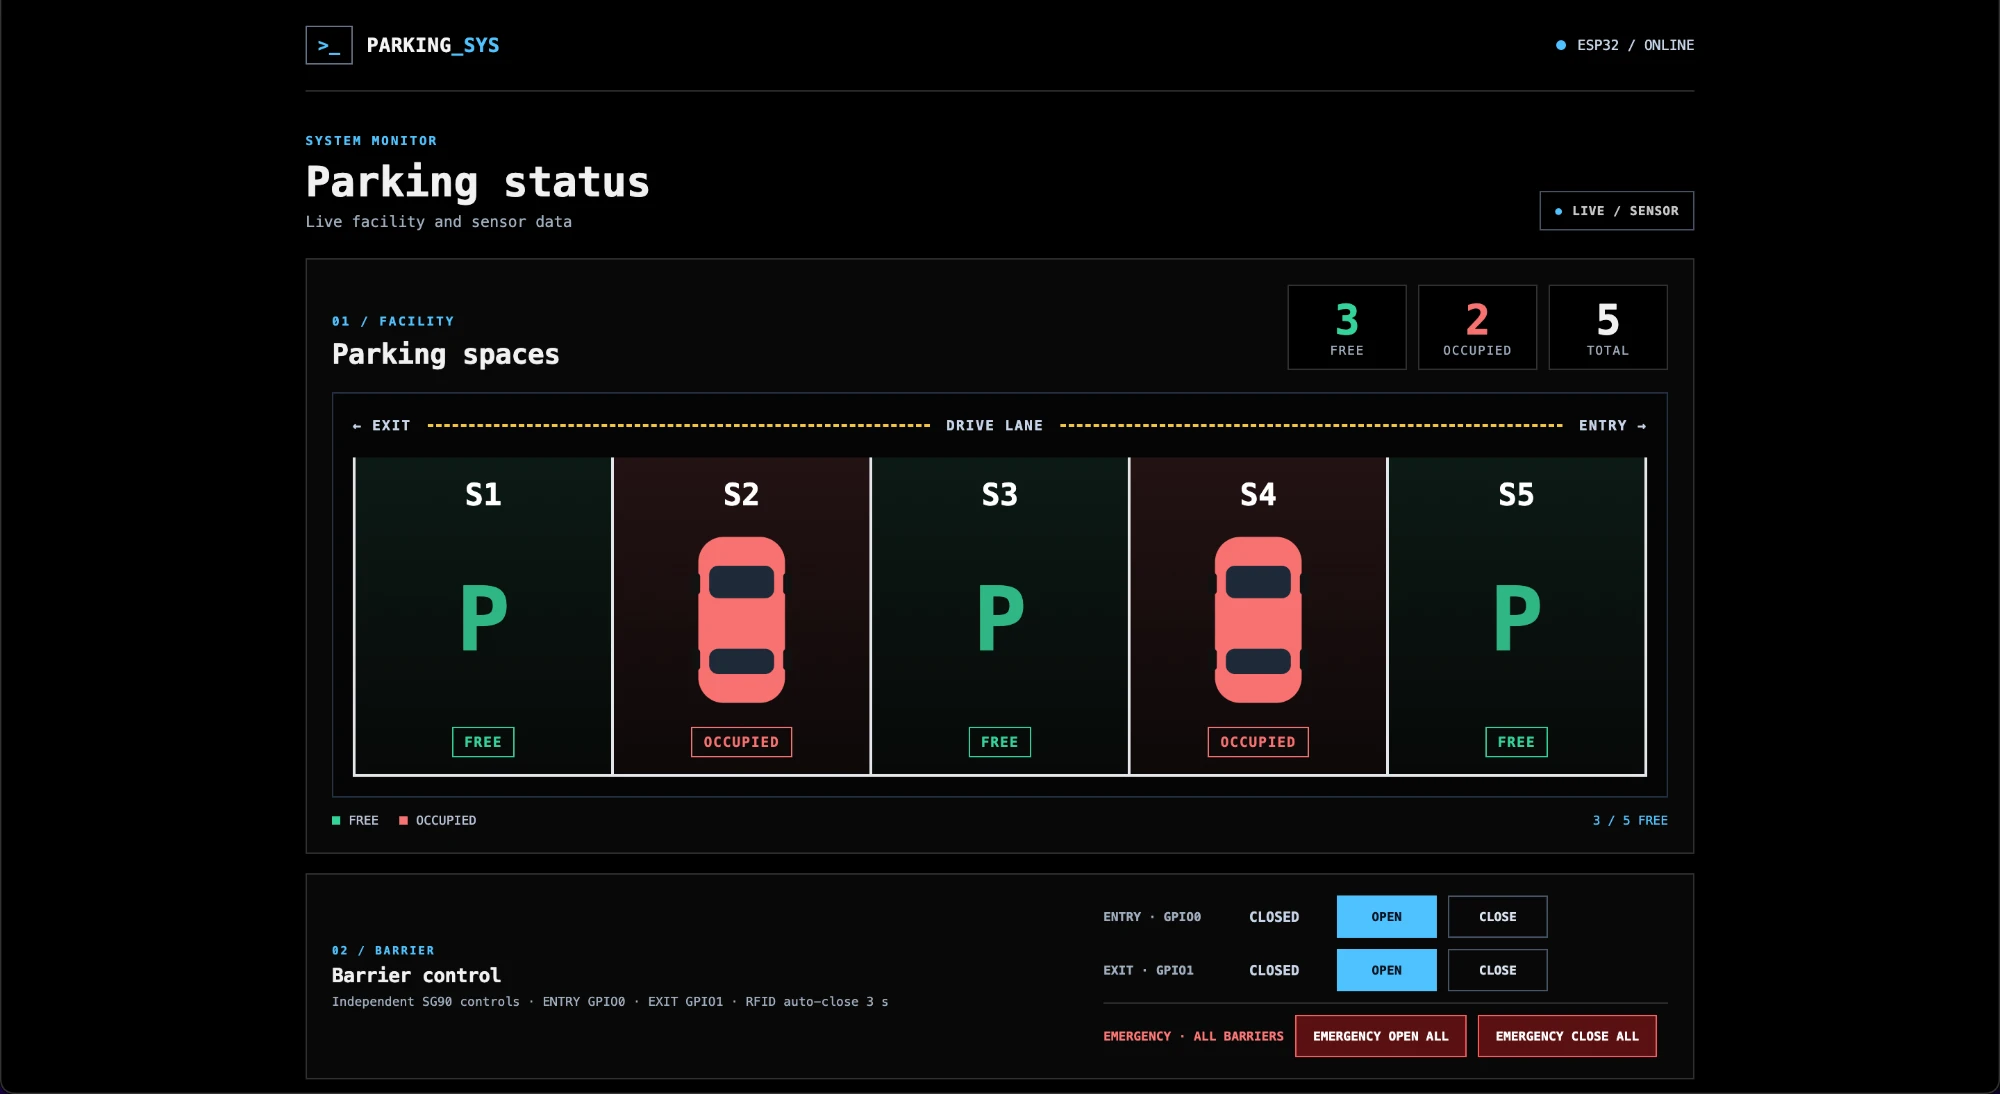
\includegraphics[width=0.9\linewidth]{photos/web_status.png}
\caption{Trang web quản lý: sơ đồ bãi và điều khiển thanh chắn}\label{fig:web-status}
\end{figure}

Trong Hình~\ref{fig:web-status}, phần chính là sơ đồ năm ô đỗ theo đúng bố cục của mô hình, với
làn xe, hướng vào và hướng ra; ô có xe được vẽ hình xe màu đỏ, ô trống hiện chữ P màu xanh. Ba ô
số ở góc trên phải cho biết số chỗ trống, số chỗ có xe và tổng số chỗ, trùng khớp với màn hình
TFT cùng thời điểm ở Hình~\ref{fig:tft-live}. Phần dưới là các nút điều khiển của UC05.

Nhiệt độ hiển thị trên trang web và màn hình đến từ RFID Client. Client đọc cảm biến DHT11 mỗi
5\,s, vì DHT11 cần tối thiểu 1\,s giữa hai lần đọc và nhiệt độ môi trường thay đổi chậm, rồi gửi
bản tin \code{climate} độc lập với việc có xe quẹt thẻ hay không. Nếu DHT11 trả về giá trị lỗi,
client giữ giá trị hợp lệ gần nhất thay vì gửi số sai. Trang web được viết bằng HTML, CSS và
JavaScript thuần, dùng phương pháp hỏi vòng thay vì WebSocket để máy chủ không phải giữ trạng
thái kết nối cho mỗi trình duyệt.

\section{UC09. Tra cứu nhật ký và doanh thu}\label{sec:uc09}
Use case này cung cấp cho người vận hành công cụ đối soát lượt xe và tiền thu được. Đặc tả được
trình bày ở Bảng~\ref{tab:uc09}.

\begin{ucspec}{Đặc tả UC09. Tra cứu nhật ký và doanh thu}{tab:uc09}
Tác nhân chính & Người vận hành \\ \midrule
Mục tiêu & Đối soát xe đang trong bãi, các sự kiện gần nhất và doanh thu \\ \midrule
Tiền điều kiện & Thiết bị của người vận hành ở cùng mạng Wi-Fi với máy chủ \\ \midrule
Kích hoạt & Người vận hành mở phần nhật ký trên trang web \\ \midrule
Luồng chính &
\bul Trang web gọi \code{GET /api/rfid} mỗi 2\,s.
\bul Máy chủ trả đơn giá, danh sách xe trong bãi kèm giờ vào và phí tạm tính, 10 sự kiện gần nhất và doanh thu.
\bul Trang web hiển thị doanh thu, số lượt vào và ra trong ngày và trong 7 ngày gần nhất. \\ \midrule
Luồng ngoại lệ &
\bul Máy chủ vừa khởi động lại sau mất điện: dữ liệu được khôi phục từ flash; khi trình duyệt gửi giờ thực, các mốc thời gian được hiệu chỉnh và thời gian mất điện được bù. \\ \midrule
Hậu điều kiện & Người vận hành có số liệu để đối chiếu với tiền thực thu \\
\end{ucspec}

Hình~\ref{fig:web-log} là phần trang web tương ứng với use case này.

\begin{figure}[H]
\centering
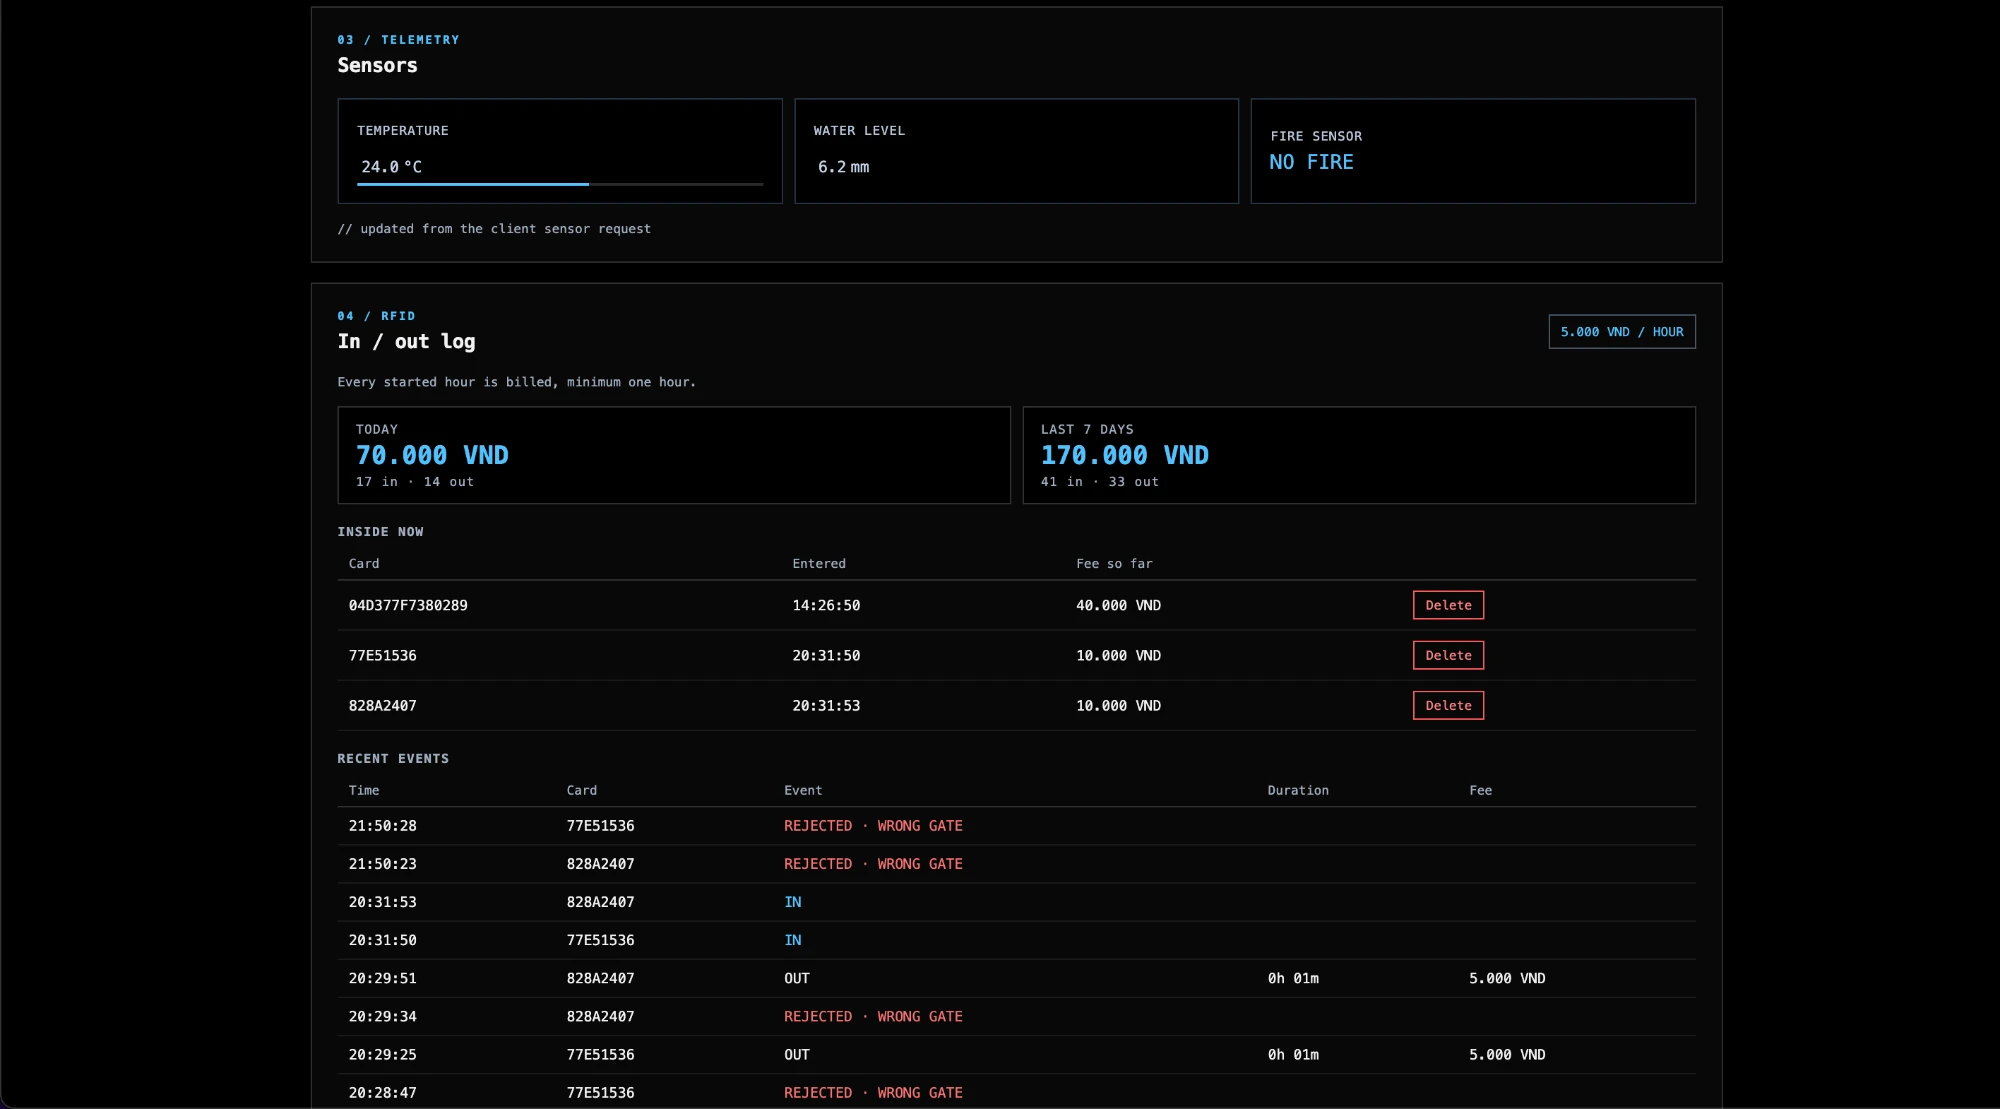
\includegraphics[width=\linewidth]{photos/web_log.png}
\caption{Trang web quản lý: cảm biến, doanh thu và nhật ký vào ra}\label{fig:web-log}
\end{figure}

Hình~\ref{fig:web-log} gồm bốn khối. Khối cảm biến hiển thị nhiệt độ, mực nước và trạng thái
cảm biến lửa. Khối doanh thu cho biết tổng tiền, số lượt vào và số lượt ra trong ngày theo giờ
Việt Nam và trong 7 ngày gần nhất. Bảng \code{INSIDE NOW} liệt kê các xe đang trong bãi; bảng
\code{RECENT EVENTS} liệt kê 10 sự kiện gần nhất gồm xe vào, xe ra kèm thời lượng và phí, và các
lần quẹt bị từ chối. Nhật ký được lưu trong bộ đệm vòng 10 phần tử, dưới 1\,KB RAM và không dùng
heap.

Toàn bộ phiên gửi xe, nhật ký, doanh thu và đồng hồ được lưu vào vùng NVS trên flash sau mỗi lần
quẹt thẻ và định kỳ 5 phút. Với khoảng 300 lần ghi mỗi ngày và cơ chế rải đều lượt ghi của NVS,
tuổi thọ flash không bị ảnh hưởng đáng kể. Máy chủ không có đồng hồ thời gian thực; trình duyệt
của người vận hành gửi giờ thực qua \code{POST /api/time}, và máy chủ dời các mốc thời gian cũ
theo đó.

\section{UC10. Hiệu chỉnh danh sách xe trong bãi}\label{sec:uc10}
Trong vận hành thực tế, danh sách xe trong bãi có thể lệch với thực tế, chẳng hạn khi xe đã rời
bãi trong lúc sơ tán cháy mà không quẹt thẻ ra, hoặc khi khách làm mất thẻ. Use case này cho phép
người vận hành sửa danh sách; đặc tả được trình bày ở Bảng~\ref{tab:uc10}.

\begin{ucspec}{Đặc tả UC10. Hiệu chỉnh danh sách xe trong bãi}{tab:uc10}
Tác nhân chính & Người vận hành \\ \midrule
Mục tiêu & Xóa một xe không còn trong bãi khỏi danh sách \\ \midrule
Tiền điều kiện & Xe có trong danh sách \code{INSIDE NOW}; người vận hành có mã PIN quản trị \\ \midrule
Kích hoạt & Người vận hành bấm \code{Delete} ở dòng của xe và xác nhận \\ \midrule
Luồng chính &
\bul Trang web gửi \code{POST /api/rfid/remove} kèm mã thẻ và mã PIN.
\bul Máy chủ xóa phiên của thẻ và hủy lượt thanh toán đang chờ của xe đó nếu có.
\bul Danh sách được lưu lại vào flash; trang web cập nhật bảng \code{INSIDE NOW}. \\ \midrule
Luồng ngoại lệ &
\bul Thẻ không có trong danh sách: máy chủ trả mã 404.
\bul Sai hoặc thiếu mã PIN: máy chủ trả mã 401. \\ \midrule
Hậu điều kiện & Thẻ có thể dùng để gửi xe lại; không có phí, hóa đơn hay thay đổi doanh thu; thanh chắn không chuyển động \\
\end{ucspec}

Theo Bảng~\ref{tab:uc10}, thao tác xóa được thiết kế khác hẳn UC04: không tính phí và không mở
thanh chắn, vì mục đích là sửa dữ liệu chứ không phải cho xe ra. Sau khi xóa, số thẻ trong bãi
khớp lại với số ô có xe theo cảm biến, nên cảnh báo xe không quẹt thẻ của UC02 và điều kiện bãi
đầy được tính đúng trở lại. Do thao tác không để lại dấu vết trong nhật ký, việc yêu cầu mã PIN
là bắt buộc.
